% ! Tex program = xelatex
\documentclass{article}
% 中文
% \usepackage[UTF8]{ctex}

% For more choices
% %! Tex program = xelatex
% \documentclass{article}
%中文
%\usepackage[UTF8]{ctex}
%数学公式
\usepackage{amsmath,amssymb}
%\usepackage{ntheorem}
% \usepackage[framemethod=TikZ]{mdframed}
\usepackage{amsthm}
%边界
\usepackage[letterpaper,top=2cm,bottom=3cm,left=2cm,right=2cm,marginparwidth=1.75cm]{geometry}%table package
%Table
\usepackage{multirow,booktabs}
\usepackage{makecell}
%字体颜色
\usepackage{color}
% \usepackage[dvipsnames]{xcolor}  % 更全的色系
%代码
\usepackage[OT1]{fontenc}
% MATLAB 代码风格
%\usepackage[framed,numbered,autolinebreaks,useliterate]{/Users/anye_zhenhaoyu/Desktop/Latex/mcode}
\usepackage{listings}
\usepackage{algorithm}
\usepackage{algorithmic}
\usepackage{pythonhighlight} % Python
%插图
\usepackage{graphicx}
%改变item格式
\usepackage{enumerate}
%物理
\usepackage{physics}
%extra arrows
\usepackage{extarrows}
% caption(居中指令)
%\usepackage[justification=centering]{caption}
\usepackage{caption}
% htpb
\usepackage{stfloats}
% pdf 拼接
\usepackage{pdfpages}
% 超链接url
\usepackage{url}
\usepackage{tikz}
\usepackage{pgfplots}
\pgfplotsset{compat=newest}
\usepackage[colorlinks=true, allcolors=red]{hyperref}
\usepackage{setspace}
\usepackage{bbm}

% --------------definations-------------- %
\def\*#1{\boldsymbol{#1}}
\def\+#1{\mathcal{#1}} 
\def\-#1{\mathrm{#1}}
\def\rm#1{\mathrm{#1}}
\def\=#1{\mathbb{#1}}
% Domains
\def\RR{\mathbb{R}}
\def\EE{\mathbb{E}}
\def\CC{\mathbb{C}}
\def\NN{\mathbb{N}}
\def\ZZ{\mathbb{Z}}
% Newcommand
\newcommand{\inner}[2]{\langle #1,#2\rangle} 
\newcommand{\numP}{\#\mathbf{P}} 
\renewcommand{\P}{\mathbf{P}}
\newcommand{\Var}[2][]{\mathbf{Var}_{#1}\left[#2\right]}
\newcommand{\E}[2][]{\mathbf{E}_{#1}\left[#2\right]}
\renewcommand{\emptyset}{\varnothing}
\newcommand{\ol}{\overline}
\newcommand{\argmin}{\mathop{\arg\min}}
\newcommand{\argmax}{\mathop{\arg\max}}
\renewcommand{\abs}[1]{\qty|#1|}
\newcommand{\defeq}{\triangleq} % triangle over =
\def\deq{\xlongequal{def}} % 'def' over =
\def\LHS{\text{LHS}}
\def\RHS{\text{RHS}}
\def\angbr#1{\langle#1\rangle} % <x>
\def\set#1{\qty{#1}}

\def\Esolve{\textcolor{blue}{Solve: }}
\def\Eproof{\textcolor{blue}{Proof: }}
\def\case#1{\textcolor{blue}{Case \uppercase\expandafter{\romannumeral#1}: }}

% \newmdtheoremenv{lemma}{Lemma}
% \newmdtheoremenv{theorem}{\textcolor{red}{Theorem}}
% \newmdtheoremenv{defi}{\textcolor{blue}{Definition}}
\newtheorem{lemma}{Lemma}
\newtheorem{thm}{Theorem}
\newtheorem{defi}{Definition}
\newtheorem{prp}{Proposition}
\newtheorem{remark}{Remark}
\newenvironment{md}{\begin{mdframed}}{\end{mdframed}}

\graphicspath{{figures/}}

% \begin{document}
% \title{<++>}
\author{Haoyu Zhen}
% \maketitle
\setlength{\parindent}{0pt}
\setstretch{1.2}
% \end{document}

\usepackage{fancyhdr}
\pagestyle{fancy}
% \fancypagestyle{mainFancy}{
%     \fancyhf{}
%     \renewcommand\headrulewidth{.5pt}       % 页眉横线
%     \renewcommand\footrulewidth{0pt}
%     \fancyhead[OC]{\fzkai{\leftmark}}       % 页眉章标题
%     \fancyhead[EC]{\fzkai{\@title}}         % 页眉文章题目
% 	\lhead{\fzkai{author}}
%     \fancyhead[OR,EL]{\thepage}                 % 页眉编号
%     \fancyfoot[r]{\thumb} % 将拇指放到没有被使用的页眉或页脚处
% }
\fancyhf{}
\fancyfoot[C]{\thepage}
\fancyhead[R]{\slshape{AI2615 Algorithm Design and Analysis}}
\fancyhead[L]{\slshape{Haoyu Zhen}}

% % theorems
\usepackage{thmtools}
\usepackage{thm-restate}
\usepackage[framemethod=TikZ]{mdframed}
\mdfsetup{skipabove=1em,skipbelow=0em, innertopmargin=12pt, innerbottommargin=8pt}

\theoremstyle{definition}

\declaretheoremstyle[headfont=\bfseries\sffamily, bodyfont=\normalfont,
	mdframed={
		nobreak,
		backgroundcolor=brown!14,
		topline=false,
		rightline=false,
		leftline=true,
		bottomline=false,
		linewidth=2pt,
		linecolor=brown!180,
	}
]{thmbrownbox}

\declaretheoremstyle[headfont=\bfseries\sffamily, bodyfont=\normalfont,
	mdframed={
		nobreak,
		backgroundcolor=Blue!4,
		topline=false,
		rightline=false,
		leftline=true,
		bottomline=false,
		linewidth=2pt,
		linecolor=NavyBlue!120,
	}
]{thmbluebox}

\declaretheoremstyle[headfont=\bfseries\sffamily, bodyfont=\normalfont,
	mdframed={
		nobreak,
		backgroundcolor=Green!5,
		topline=false,
		rightline=false,
		leftline=true,
		bottomline=false,
		linewidth=2pt,
		linecolor=OliveGreen!120,
	}
]{thmgreenbox}

\declaretheoremstyle[headfont=\bfseries\sffamily, bodyfont=\normalfont,
	mdframed={
		nobreak,
		topline=false,
		rightline=false,
		leftline=true,
		bottomline=false,
		linewidth=2pt,
		linecolor=OliveGreen!120,
	}
]{thmgreenline}

\declaretheoremstyle[headfont=\bfseries\sffamily, bodyfont=\normalfont,
	mdframed={
		nobreak,
		topline=false,
		rightline=false,
		leftline=true,
		bottomline=false,
		linewidth=2pt,
		linecolor=NavyBlue!70,
	}
]{thmblueline}

\declaretheorem[numberwithin=section, style=thmbrownbox, name={\color{Brown}Definition}]{defi}
\declaretheorem[numberwithin=section, style=thmgreenbox, name={\color{OliveGreen}Law}]{law}
\declaretheorem[numberwithin=section, style=thmbluebox, name={\color{Blue}Corollary}]{cor}
\declaretheorem[numberwithin=section, style=thmgreenline, name={\color{OliveGreen}Property}]{prt}
\declaretheorem[numberwithin=section, style=thmbluebox, name={\color{Blue}Proposition}]{prp}
\declaretheorem[numberwithin=section, style=thmbluebox, name={\color{Blue}Theorem}]{thm}
\declaretheorem[numberwithin=section, style=thmbluebox, name={\color{Blue}Lemma}]{lemma}
\declaretheorem[numberwithin=section, style=thmbrownbox,  name={\color{Brown}Example}]{eg}
\declaretheorem[numberwithin=section, style=thmgreenline, name={\color{OliveGreen}Remark}]{remark}
\declaretheorem[numbered=no,style=thmblueline, name={\color{NavyBlue!70}Proof},qed=$\square$]{prf}
\numberwithin{equation}{section}


% %! Tex program = xelatex
% \documentclass{article}
%中文
%\usepackage[UTF8]{ctex}
%数学公式
\usepackage{amsmath,amssymb}
%\usepackage{ntheorem}
% \usepackage[framemethod=TikZ]{mdframed}
\usepackage{amsthm}
%边界
\usepackage[letterpaper,top=2cm,bottom=3cm,left=2cm,right=2cm,marginparwidth=1.75cm]{geometry}%table package
%Table
\usepackage{multirow,booktabs}
\usepackage{makecell}
%字体颜色
\usepackage{color}
% \usepackage[dvipsnames]{xcolor}  % 更全的色系
%代码
\usepackage[OT1]{fontenc}
% MATLAB 代码风格
%\usepackage[framed,numbered,autolinebreaks,useliterate]{/Users/anye_zhenhaoyu/Desktop/Latex/mcode}
\usepackage{listings}
\usepackage{algorithm}
\usepackage{algorithmic}
\usepackage{pythonhighlight} % Python
%插图
\usepackage{graphicx}
%改变item格式
\usepackage{enumerate}
%物理
\usepackage{physics}
%extra arrows
\usepackage{extarrows}
% caption(居中指令)
%\usepackage[justification=centering]{caption}
\usepackage{caption}
% htpb
\usepackage{stfloats}
% pdf 拼接
\usepackage{pdfpages}
% 超链接url
\usepackage{url}
\usepackage{tikz}
\usepackage{pgfplots}
\pgfplotsset{compat=newest}
\usepackage[colorlinks=true, allcolors=red]{hyperref}
\usepackage{setspace}
\usepackage{bbm}

% --------------definations-------------- %
\def\*#1{\boldsymbol{#1}}
\def\+#1{\mathcal{#1}} 
\def\-#1{\mathrm{#1}}
\def\rm#1{\mathrm{#1}}
\def\=#1{\mathbb{#1}}
% Domains
\def\RR{\mathbb{R}}
\def\EE{\mathbb{E}}
\def\CC{\mathbb{C}}
\def\NN{\mathbb{N}}
\def\ZZ{\mathbb{Z}}
% Newcommand
\newcommand{\inner}[2]{\langle #1,#2\rangle} 
\newcommand{\numP}{\#\mathbf{P}} 
\renewcommand{\P}{\mathbf{P}}
\newcommand{\Var}[2][]{\mathbf{Var}_{#1}\left[#2\right]}
\newcommand{\E}[2][]{\mathbf{E}_{#1}\left[#2\right]}
\renewcommand{\emptyset}{\varnothing}
\newcommand{\ol}{\overline}
\newcommand{\argmin}{\mathop{\arg\min}}
\newcommand{\argmax}{\mathop{\arg\max}}
\renewcommand{\abs}[1]{\qty|#1|}
\newcommand{\defeq}{\triangleq} % triangle over =
\def\deq{\xlongequal{def}} % 'def' over =
\def\LHS{\text{LHS}}
\def\RHS{\text{RHS}}
\def\angbr#1{\langle#1\rangle} % <x>
\def\set#1{\qty{#1}}

\def\Esolve{\textcolor{blue}{Solve: }}
\def\Eproof{\textcolor{blue}{Proof: }}
\def\case#1{\textcolor{blue}{Case \uppercase\expandafter{\romannumeral#1}: }}

% \newmdtheoremenv{lemma}{Lemma}
% \newmdtheoremenv{theorem}{\textcolor{red}{Theorem}}
% \newmdtheoremenv{defi}{\textcolor{blue}{Definition}}
\newtheorem{lemma}{Lemma}
\newtheorem{thm}{Theorem}
\newtheorem{defi}{Definition}
\newtheorem{prp}{Proposition}
\newtheorem{remark}{Remark}
\newenvironment{md}{\begin{mdframed}}{\end{mdframed}}

\graphicspath{{figures/}}

% \begin{document}
% \title{<++>}
\author{Haoyu Zhen}
% \maketitle
\setlength{\parindent}{0pt}
\setstretch{1.2}
% \end{document}

\usepackage{fancyhdr}
\pagestyle{fancy}
% \fancypagestyle{mainFancy}{
%     \fancyhf{}
%     \renewcommand\headrulewidth{.5pt}       % 页眉横线
%     \renewcommand\footrulewidth{0pt}
%     \fancyhead[OC]{\fzkai{\leftmark}}       % 页眉章标题
%     \fancyhead[EC]{\fzkai{\@title}}         % 页眉文章题目
% 	\lhead{\fzkai{author}}
%     \fancyhead[OR,EL]{\thepage}                 % 页眉编号
%     \fancyfoot[r]{\thumb} % 将拇指放到没有被使用的页眉或页脚处
% }
\fancyhf{}
\fancyfoot[C]{\thepage}
\fancyhead[R]{\slshape{AI2615 Algorithm Design and Analysis}}
\fancyhead[L]{\slshape{Haoyu Zhen}}

% % theorems
\usepackage{thmtools}
\usepackage{thm-restate}
\usepackage[framemethod=TikZ]{mdframed}
\mdfsetup{skipabove=1em,skipbelow=0em, innertopmargin=12pt, innerbottommargin=8pt}

\theoremstyle{definition}

\declaretheoremstyle[headfont=\bfseries\sffamily, bodyfont=\normalfont,
	mdframed={
		nobreak,
		backgroundcolor=brown!14,
		topline=false,
		rightline=false,
		leftline=true,
		bottomline=false,
		linewidth=2pt,
		linecolor=brown!180,
	}
]{thmbrownbox}

\declaretheoremstyle[headfont=\bfseries\sffamily, bodyfont=\normalfont,
	mdframed={
		nobreak,
		backgroundcolor=Blue!4,
		topline=false,
		rightline=false,
		leftline=true,
		bottomline=false,
		linewidth=2pt,
		linecolor=NavyBlue!120,
	}
]{thmbluebox}

\declaretheoremstyle[headfont=\bfseries\sffamily, bodyfont=\normalfont,
	mdframed={
		nobreak,
		backgroundcolor=Green!5,
		topline=false,
		rightline=false,
		leftline=true,
		bottomline=false,
		linewidth=2pt,
		linecolor=OliveGreen!120,
	}
]{thmgreenbox}

\declaretheoremstyle[headfont=\bfseries\sffamily, bodyfont=\normalfont,
	mdframed={
		nobreak,
		topline=false,
		rightline=false,
		leftline=true,
		bottomline=false,
		linewidth=2pt,
		linecolor=OliveGreen!120,
	}
]{thmgreenline}

\declaretheoremstyle[headfont=\bfseries\sffamily, bodyfont=\normalfont,
	mdframed={
		nobreak,
		topline=false,
		rightline=false,
		leftline=true,
		bottomline=false,
		linewidth=2pt,
		linecolor=NavyBlue!70,
	}
]{thmblueline}

\declaretheorem[numberwithin=section, style=thmbrownbox, name={\color{Brown}Definition}]{defi}
\declaretheorem[numberwithin=section, style=thmgreenbox, name={\color{OliveGreen}Law}]{law}
\declaretheorem[numberwithin=section, style=thmbluebox, name={\color{Blue}Corollary}]{cor}
\declaretheorem[numberwithin=section, style=thmgreenline, name={\color{OliveGreen}Property}]{prt}
\declaretheorem[numberwithin=section, style=thmbluebox, name={\color{Blue}Proposition}]{prp}
\declaretheorem[numberwithin=section, style=thmbluebox, name={\color{Blue}Theorem}]{thm}
\declaretheorem[numberwithin=section, style=thmbluebox, name={\color{Blue}Lemma}]{lemma}
\declaretheorem[numberwithin=section, style=thmbrownbox,  name={\color{Brown}Example}]{eg}
\declaretheorem[numberwithin=section, style=thmgreenline, name={\color{OliveGreen}Remark}]{remark}
\declaretheorem[numbered=no,style=thmblueline, name={\color{NavyBlue!70}Proof},qed=$\square$]{prf}
\numberwithin{equation}{section}


% On my MAC's Desktop
%! Tex program = xelatex
% \documentclass{article}
%中文
%\usepackage[UTF8]{ctex}
%数学公式
\usepackage{amsmath,amssymb}
%\usepackage{ntheorem}
% \usepackage[framemethod=TikZ]{mdframed}
\usepackage{amsthm}
%边界
\usepackage[letterpaper,top=2cm,bottom=3cm,left=2cm,right=2cm,marginparwidth=1.75cm]{geometry}%table package
%Table
\usepackage{multirow,booktabs}
\usepackage{makecell}
%字体颜色
\usepackage{color}
% \usepackage[dvipsnames]{xcolor}  % 更全的色系
%代码
\usepackage[OT1]{fontenc}
% MATLAB 代码风格
%\usepackage[framed,numbered,autolinebreaks,useliterate]{/Users/anye_zhenhaoyu/Desktop/Latex/mcode}
\usepackage{listings}
\usepackage{algorithm}
\usepackage{algorithmic}
\usepackage{pythonhighlight} % Python
%插图
\usepackage{graphicx}
%改变item格式
\usepackage{enumerate}
%物理
\usepackage{physics}
%extra arrows
\usepackage{extarrows}
% caption(居中指令)
%\usepackage[justification=centering]{caption}
\usepackage{caption}
% htpb
\usepackage{stfloats}
% pdf 拼接
\usepackage{pdfpages}
% 超链接url
\usepackage{url}
\usepackage{tikz}
\usepackage{pgfplots}
\pgfplotsset{compat=newest}
\usepackage[colorlinks=true, allcolors=red]{hyperref}
\usepackage{setspace}
\usepackage{bbm}

% --------------definations-------------- %
\def\*#1{\boldsymbol{#1}}
\def\+#1{\mathcal{#1}} 
\def\-#1{\mathrm{#1}}
\def\rm#1{\mathrm{#1}}
\def\=#1{\mathbb{#1}}
% Domains
\def\RR{\mathbb{R}}
\def\EE{\mathbb{E}}
\def\CC{\mathbb{C}}
\def\NN{\mathbb{N}}
\def\ZZ{\mathbb{Z}}
% Newcommand
\newcommand{\inner}[2]{\langle #1,#2\rangle} 
\newcommand{\numP}{\#\mathbf{P}} 
\renewcommand{\P}{\mathbf{P}}
\newcommand{\Var}[2][]{\mathbf{Var}_{#1}\left[#2\right]}
\newcommand{\E}[2][]{\mathbf{E}_{#1}\left[#2\right]}
\renewcommand{\emptyset}{\varnothing}
\newcommand{\ol}{\overline}
\newcommand{\argmin}{\mathop{\arg\min}}
\newcommand{\argmax}{\mathop{\arg\max}}
\renewcommand{\abs}[1]{\qty|#1|}
\newcommand{\defeq}{\triangleq} % triangle over =
\def\deq{\xlongequal{def}} % 'def' over =
\def\LHS{\text{LHS}}
\def\RHS{\text{RHS}}
\def\angbr#1{\langle#1\rangle} % <x>
\def\set#1{\qty{#1}}

\def\Esolve{\textcolor{blue}{Solve: }}
\def\Eproof{\textcolor{blue}{Proof: }}
\def\case#1{\textcolor{blue}{Case \uppercase\expandafter{\romannumeral#1}: }}

% \newmdtheoremenv{lemma}{Lemma}
% \newmdtheoremenv{theorem}{\textcolor{red}{Theorem}}
% \newmdtheoremenv{defi}{\textcolor{blue}{Definition}}
\newtheorem{lemma}{Lemma}
\newtheorem{thm}{Theorem}
\newtheorem{defi}{Definition}
\newtheorem{prp}{Proposition}
\newtheorem{remark}{Remark}
\newenvironment{md}{\begin{mdframed}}{\end{mdframed}}

\graphicspath{{figures/}}

% \begin{document}
% \title{<++>}
\author{Haoyu Zhen}
% \maketitle
\setlength{\parindent}{0pt}
\setstretch{1.2}
% \end{document}

\usepackage{fancyhdr}
\pagestyle{fancy}
% \fancypagestyle{mainFancy}{
%     \fancyhf{}
%     \renewcommand\headrulewidth{.5pt}       % 页眉横线
%     \renewcommand\footrulewidth{0pt}
%     \fancyhead[OC]{\fzkai{\leftmark}}       % 页眉章标题
%     \fancyhead[EC]{\fzkai{\@title}}         % 页眉文章题目
% 	\lhead{\fzkai{author}}
%     \fancyhead[OR,EL]{\thepage}                 % 页眉编号
%     \fancyfoot[r]{\thumb} % 将拇指放到没有被使用的页眉或页脚处
% }
\fancyhf{}
\fancyfoot[C]{\thepage}
\fancyhead[R]{\slshape{AI2615 Algorithm Design and Analysis}}
\fancyhead[L]{\slshape{Haoyu Zhen}}


\graphicspath{{../}}
\fancyhead[C]{\Large\textbf{Programming Assignment 2}}

\begin{document}
\title{Programming Assignment 2}
Code is available at ``PA2.m''. Also I superimpose the curves of spectrum for each process in Figure \ref{spectrum}, \ref{left} and \ref{head}.

\section*{Process 1}
Let $t_s=0.4$. Then $x[n]=1$ if $n\in\qty{0,1,\cdots, 25}$ otherwise $x[n]=0$.
\[
	X(\omega)
	=
	\sum_{n=-\infty}^{+\infty} x[n]e^{-j\omega n}
	=
	\sum_{n=0}^{25} e^{-j\omega n}
	=
	\frac{1-e^{26j\omega}}{1-e^{j\omega}}
.\] 
Then $\abs{X}$ reads:
 \[
	 \abs{X(\omega)}=
	 \qty|\frac{\sin{13\omega}}{\sin(\flatfrac{\omega}{2})}|
.\] 
Figure \ref{origin} and \ref{spectrum} are the diagrams of procces 1. I use $f[n]=1$ if $n\in\qty{0,1,\cdots, 101}$ to represent rectangle function $x(t)$ approximately and use \mcode{f(1:sample:end)} to sample.


\section*{Process 2}
After shiftted, $x[n]=1$ if $n\in\qty{1,2, \cdots, 25}$ otherwise $x[n]=0$.
Similarly,
\[
	\abs{X(\omega)}=
	\qty|\frac{\sin{12.5\omega}}{\sin(\flatfrac{\omega}{2})}|
.\] 
Figure \ref{shiftted} and \ref{spectrum} are the diagrams of procces 2. There are subtle differences between 1 and 2: $x[0]=1\to x[0]=0$.


\section*{Process 3}
In MATLAB, I use ``\mcode{[b,a] = butter(order, Wn); filt = filtfilt(b,a,shiftted);}'' to filter the rectangle function where $\mathrm{order}=9$ and  $\mathrm{Wn}=0.1$. Then $x(t)=\+F^{-1}\qty[\flatfrac{2\sin(5\omega)}{\omega}\cdot\mathrm{Butter}(\omega_0)]$ and 
\begin{equation}
	\begin{aligned}
		X(\omega)&=
		\+F\qty{\+F^{-1}\qty[\frac{2\sin(5\omega)}{\omega}\cdot\mathrm{Butter}(\omega_0)]
		\cdot
		\sum_{k=-\infty}^{+\infty} \delta(t-kT_s)}
	\end{aligned}
\end{equation}
This entails
\begin{equation}
	X(\omega)=\qty[\frac{2\sin(5\omega)}{\omega}\cdot\mathrm{Butter}(\omega_0)]*\qty[
			\frac{2\pi}{T_s}
			\sum_{k=-\infty}^{+\infty}
			\delta\qty(\omega-k\frac{2\pi}{T_s})
		]
	\label{p3}
\end{equation}
It is noteworthy that the Eq.\ref{p3} has no simple analytic form and $X(\omega)$ is a periodic function. However, if $\omega_0<\flatfrac{2\pi}{T_s}$, then $X(\omega)=\flatfrac{2\sin(5\omega)}{(T_s\omega)}\cdot\mathrm{Butter}(\omega_0)$ approximately.
Figure \ref{filtered} and \ref{spectrum} are the diagrams of procces 3.




\newpage
\section*{\textcolor{blue}{Appendix}}
\begin{figure}[H]
	\centering
	\begin{minipage}[b]{0.46\linewidth}
		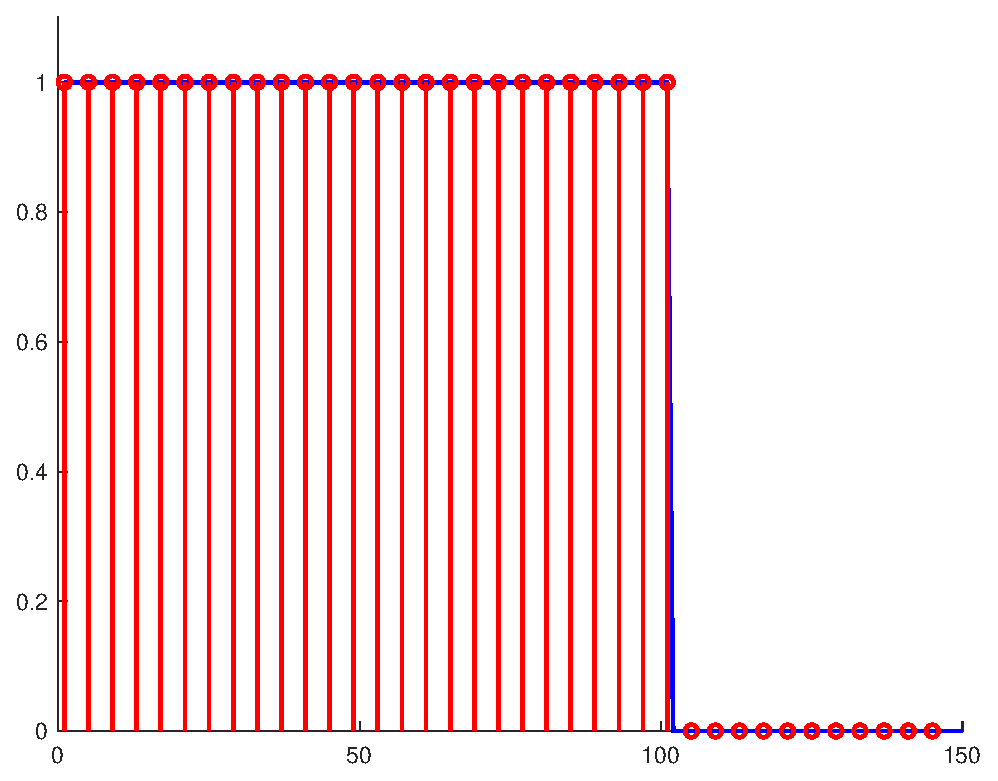
\includegraphics[width=\linewidth]{p1_time.eps}
		\caption{Original}
		\label{origin}
	\end{minipage}
	\begin{minipage}[b]{0.46\linewidth}
		\includegraphics[width=\linewidth]{p2_time.eps}
		\caption{Shiftted}
		\label{shiftted}
	\end{minipage}
	\begin{minipage}[b]{0.46\linewidth}
		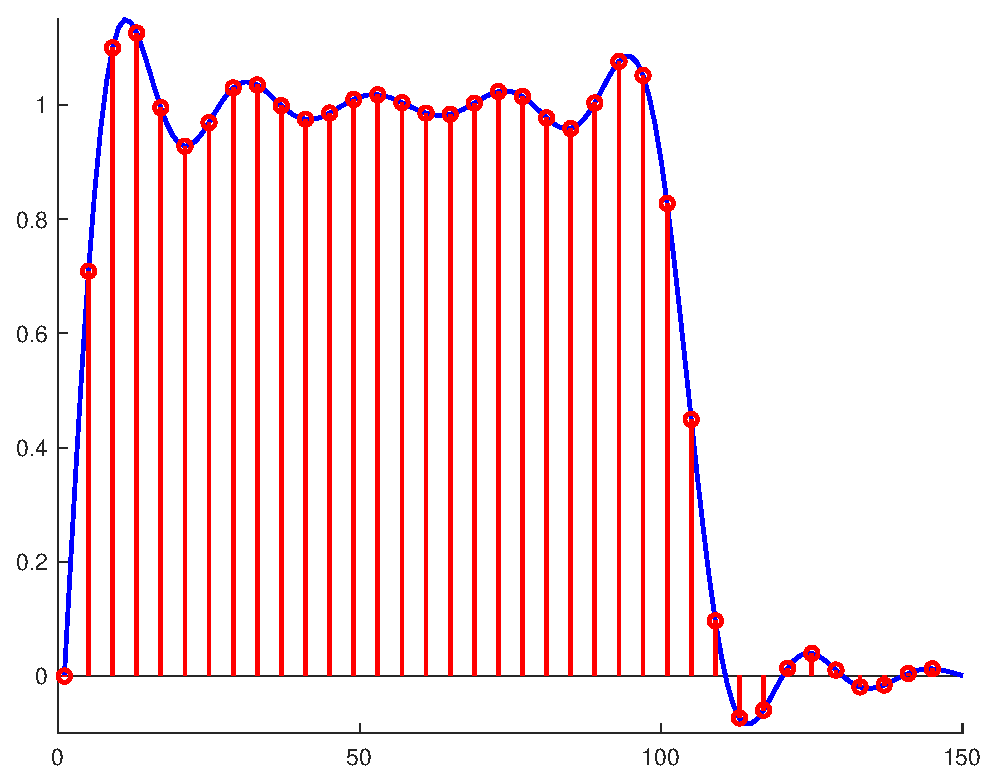
\includegraphics[width=\linewidth]{p3_time.eps}
		\caption{Filtered}
		\label{filtered}
	\end{minipage}
	\begin{minipage}[b]{0.46\linewidth}
		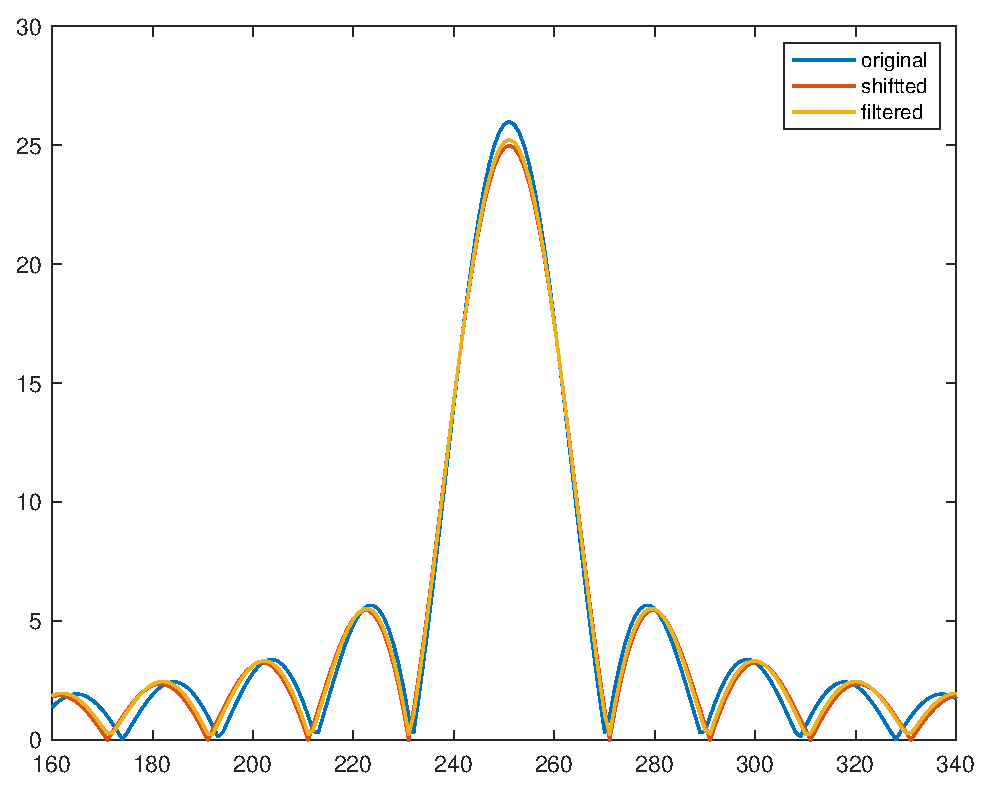
\includegraphics[width=\linewidth]{spectrum.eps}
		\caption{Spectrum}
		\label{spectrum}
	\end{minipage}
	\begin{minipage}[b]{0.46\linewidth}
		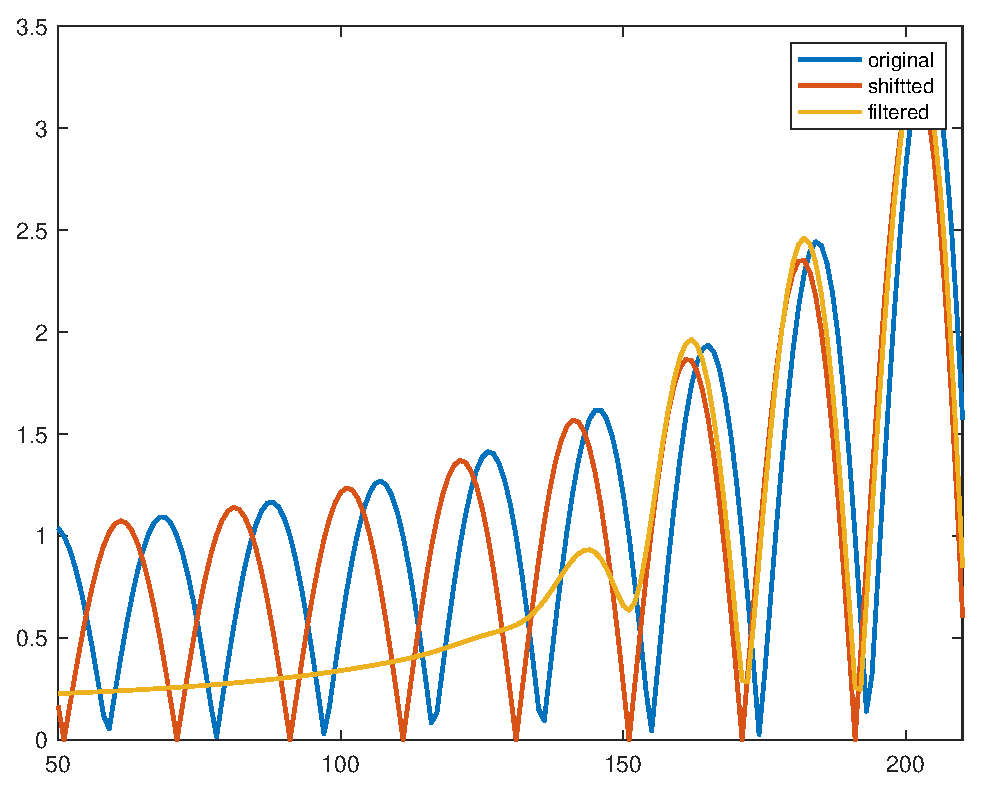
\includegraphics[width=\linewidth]{spectrum_prime.eps}
		\caption{Spectrum (Left)}
		\label{left}
	\end{minipage}
	\begin{minipage}[b]{0.46\linewidth}
		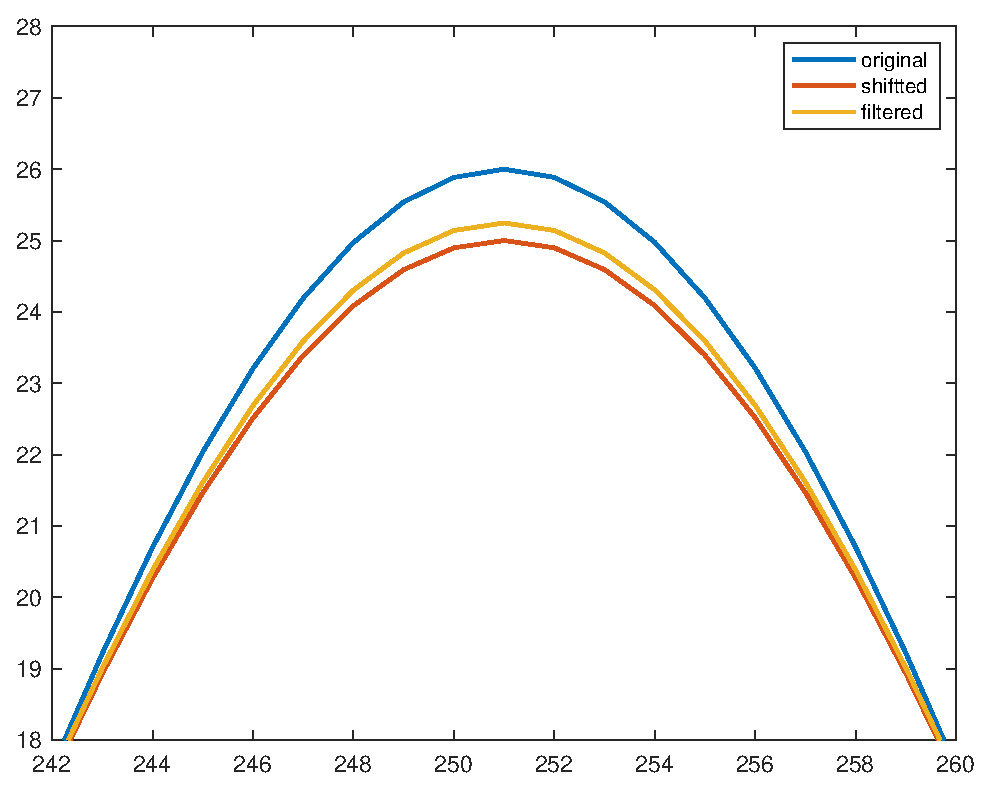
\includegraphics[width=\linewidth]{spectrum_prime2.eps}
		\caption{Spectrum (The highest peak)}
		\label{head}
	\end{minipage}
\end{figure}
\end{document}

